\documentclass[12pt, oneside]{article}
 
\usepackage{graphicx}
\usepackage{hyperref}
\graphicspath{ {../Images/} }

\begin{document}
\thispagestyle{empty}
\begin{center}
\begin{minipage}{0.9\linewidth}
    \centering


    {\normalsize Project Tender\par}
    \vspace{1cm}
    {\Large Project: DriveStats\par}
{\normalsize Client: DVT\par}
    \vspace{1cm}
   {\Large Team: Team Name\par}
    {\normalsize Renaldo van Dyk (12204359)\par}
    {\normalsize Johann Dian Marx (12105202)\par}
    {\normalsize Sean Thomas Hill (12221458)\par}
    {\normalsize Andreas du Preez (12207871)\par}
    {\normalsize Shaun Meintjes (13310896)\par}
{\normalsize Department of Computer Science, University of Pretoria\par}
    \vspace{1cm}

 {\normalsize Date: May 2015}
\vspace{1cm}
    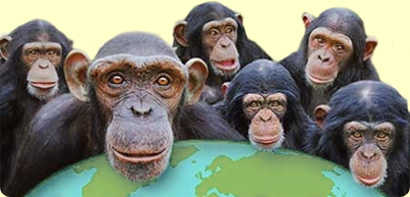
\includegraphics[scale=0.9]{example1} %Example is the name of the image

    \vspace{1cm}
    
\end{minipage}
\end{center}
\clearpage

\newpage

\section{The Team}
	\begin{enumerate}
		\item {Renaldo van Dyk (12204359)\par}
		\begin{itemize}
			\item Photo\newline
				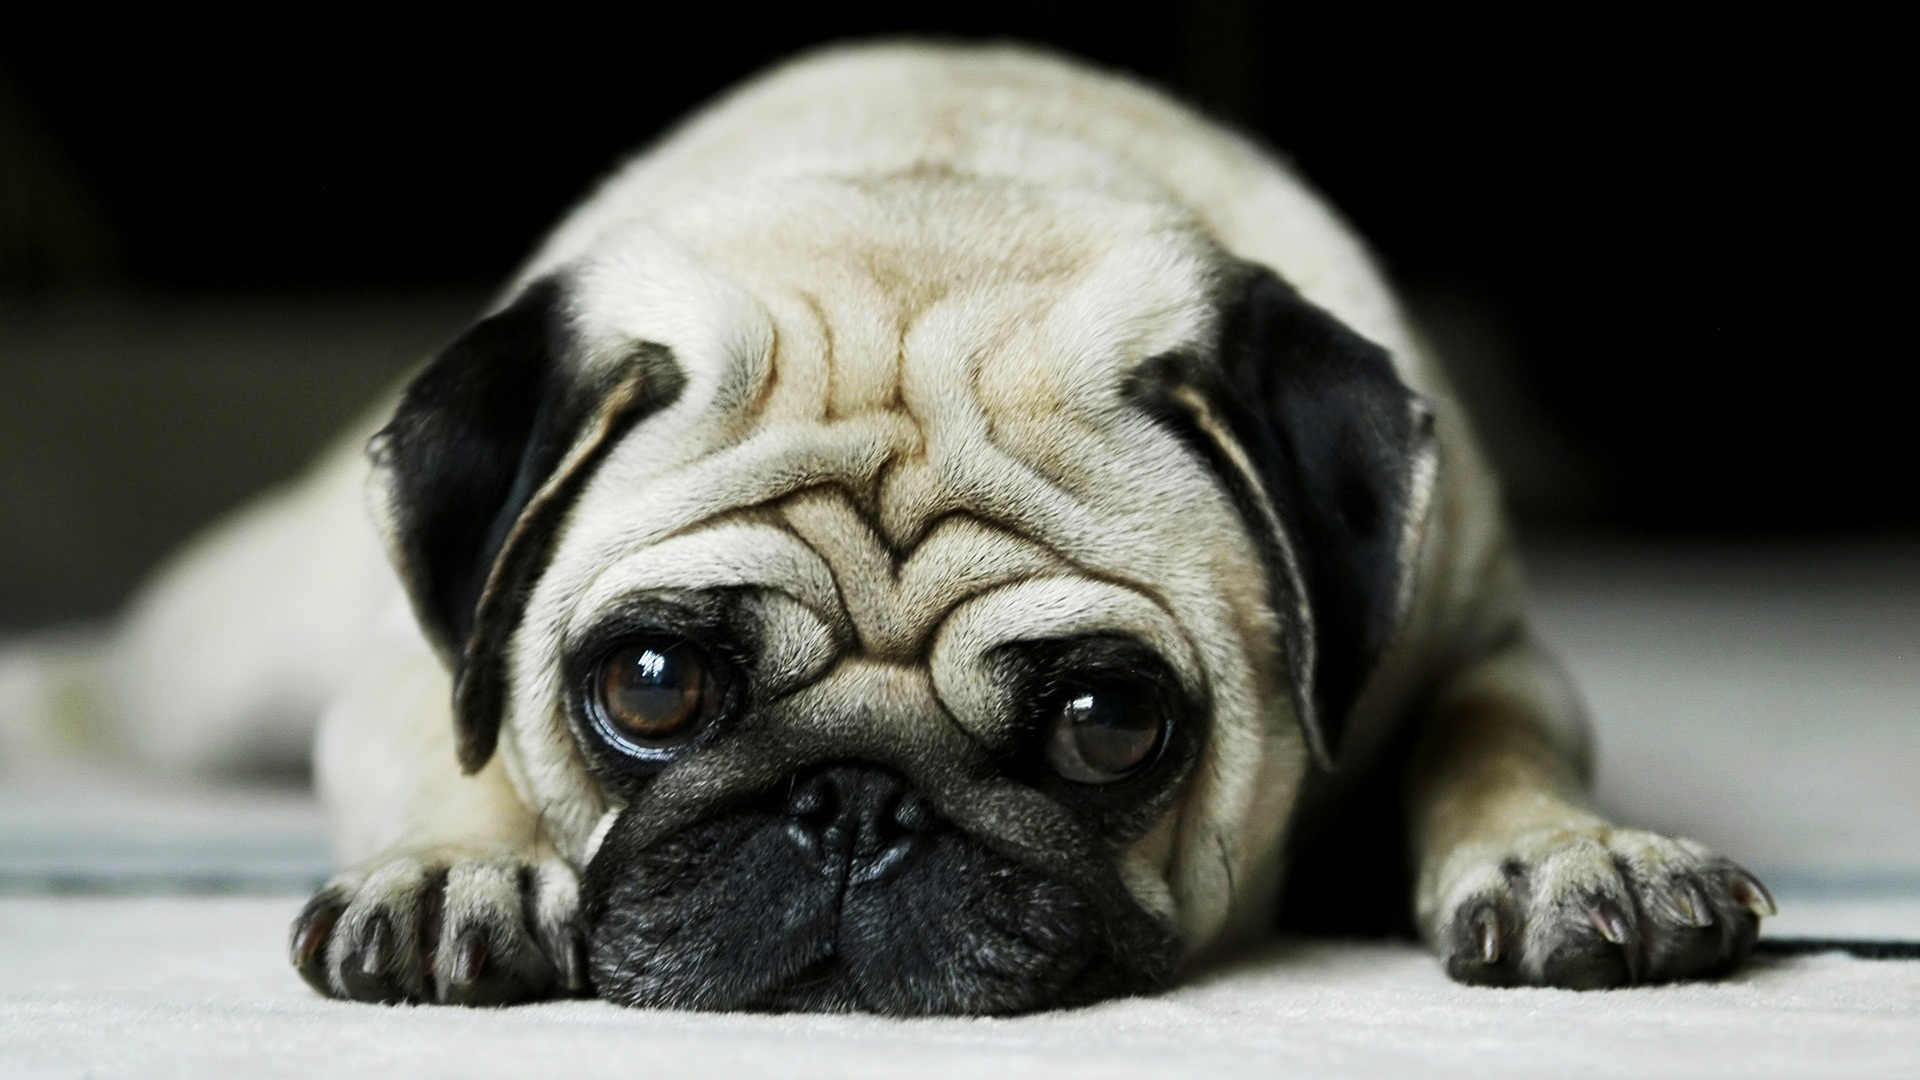
\includegraphics[scale=0.1]{example} %Example is the name of the image
			\item Interests\newline
				Fill in later...
			\item Technical Skills\newline
				Fill in later...
			\item Past experience relevant to project\newline
				Fill in later...
			\item Non-technical strengths\newline
				Fill in later...
			\item What makes you want to do the project\newline
				Fill in later...
		\end{itemize}
		\item {Johann Dian Marx (12105202)\par}
		\begin{itemize}
			\item Photo\newline
				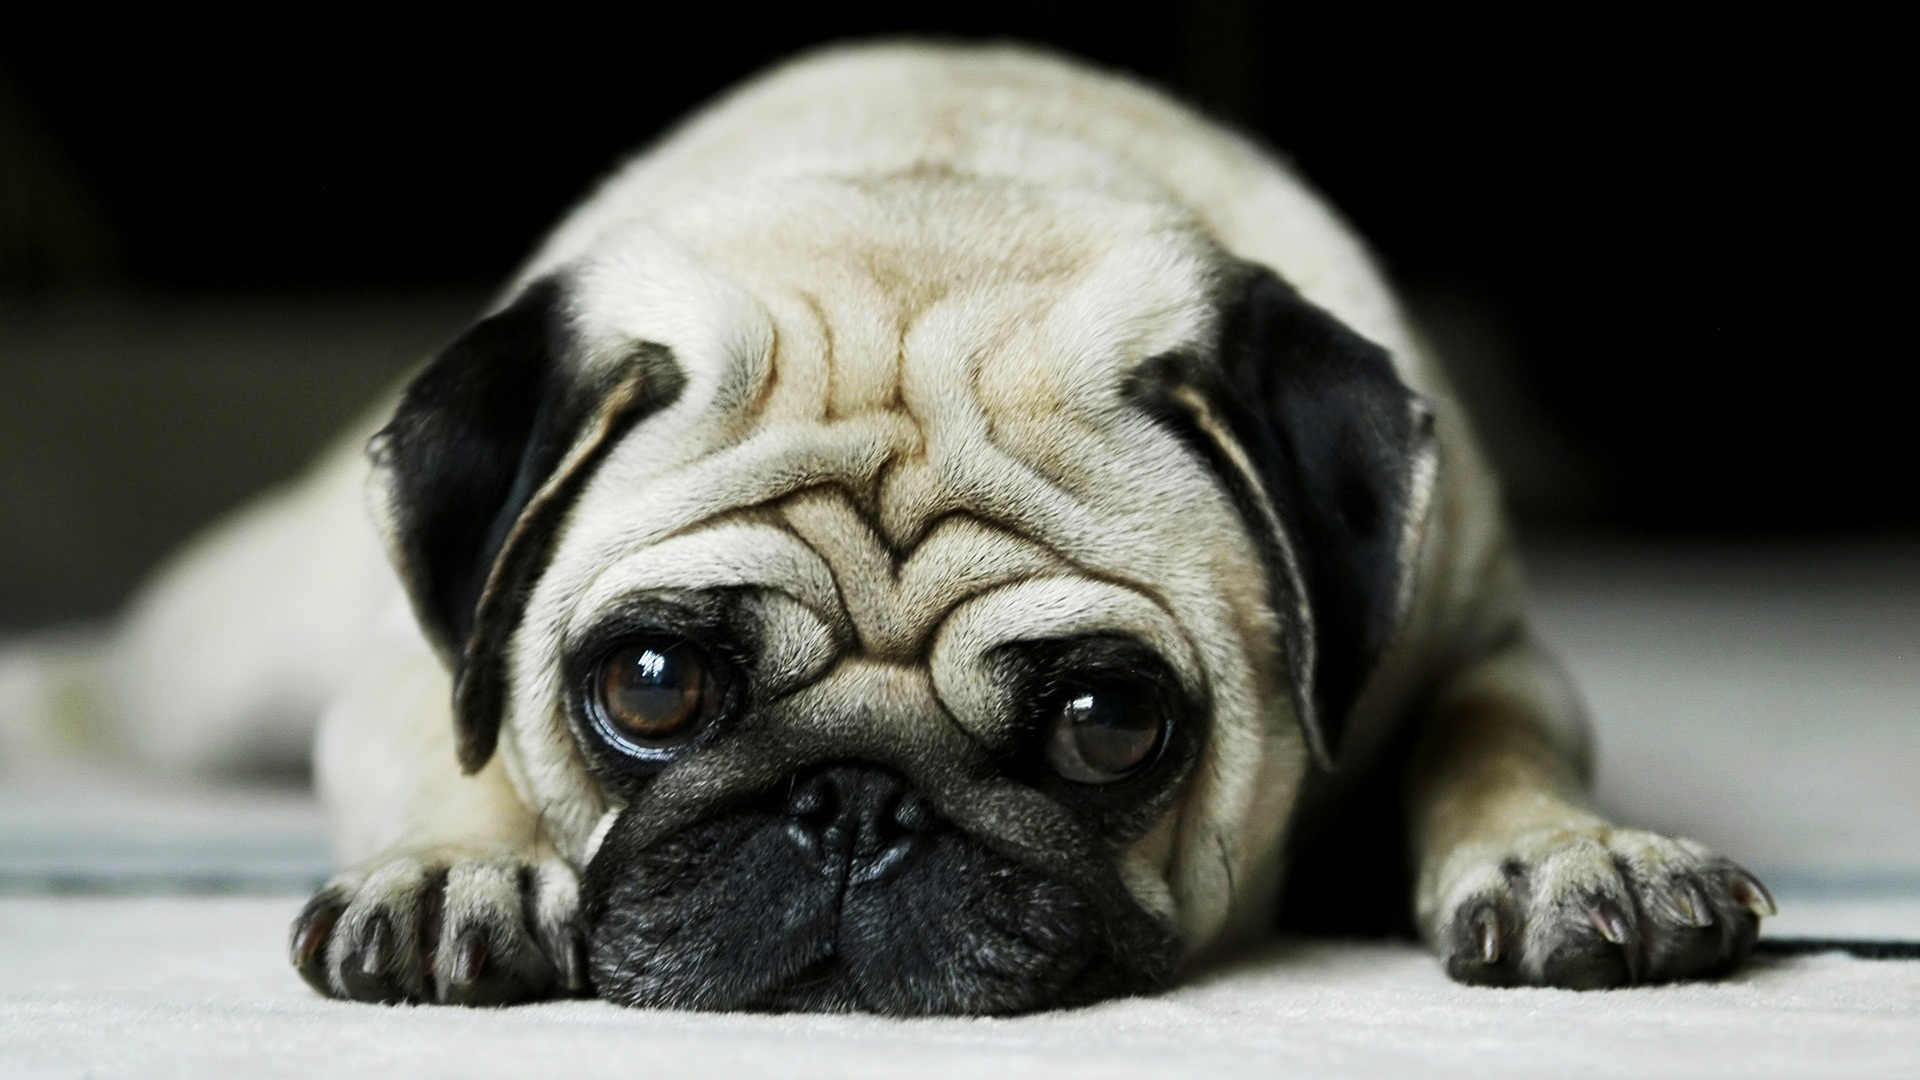
\includegraphics[scale=0.1]{example} %Example is the name of the image
			\item Interests\newline
				Fill in later...
			\item Technical Skills\newline
				Fill in later...
			\item Past experience relevant to project\newline
				Fill in later...
			\item Non-technical strengths\newline
				Fill in later...
			\item What makes you want to do the project\newline
				Fill in later...
		\end{itemize}
		\item {Sean Thomas Hill (12221458)\par}
		\begin{itemize}
			\item Photo\newline
				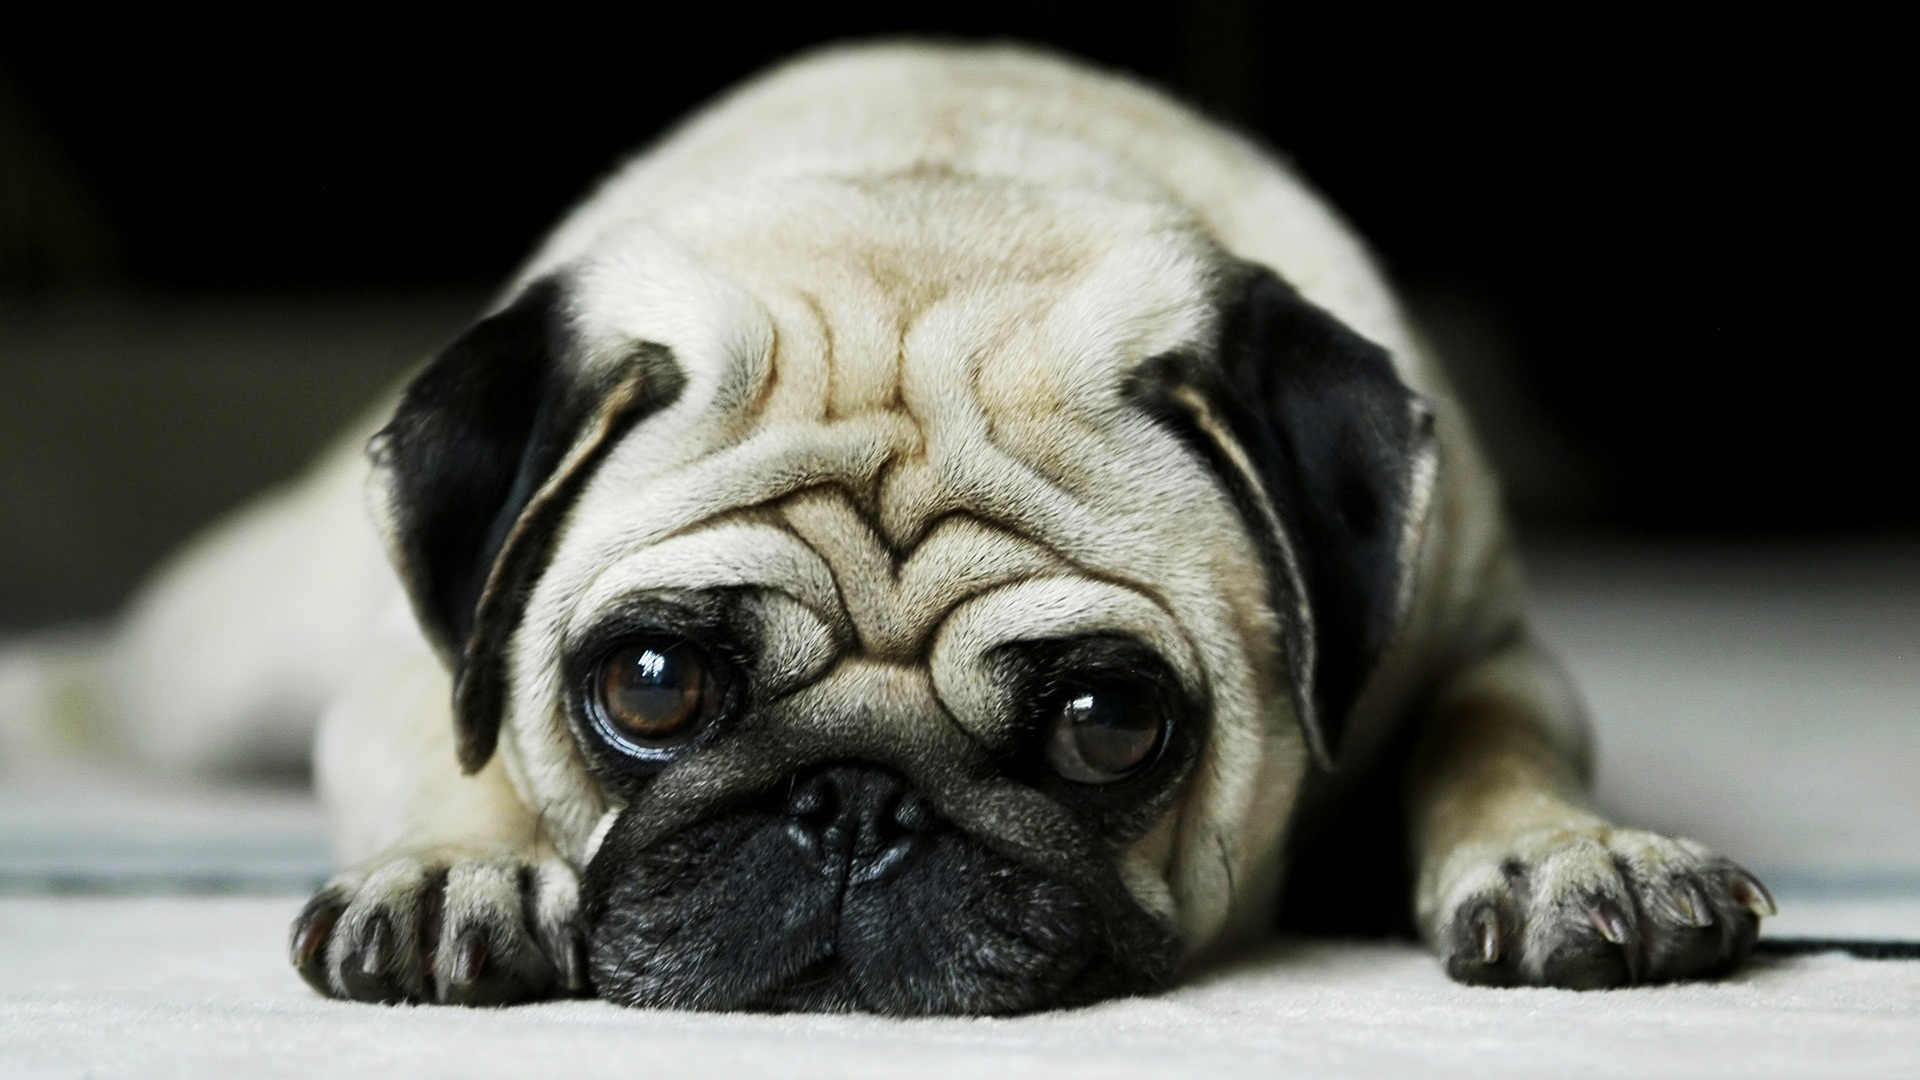
\includegraphics[scale=0.1]{example} %Example is the name of the image
			\item Interests\newline
				Fill in later...
			\item Technical Skills\newline
				Fill in later...
			\item Past experience relevant to project\newline
				Fill in later...
			\item Non-technical strengths\newline
				Fill in later...
			\item What makes you want to do the project\newline
				Fill in later...
		\end{itemize}
		\item {Andreas du Preez (12207871)\par}
		\begin{itemize}
			\item Photo\newline
				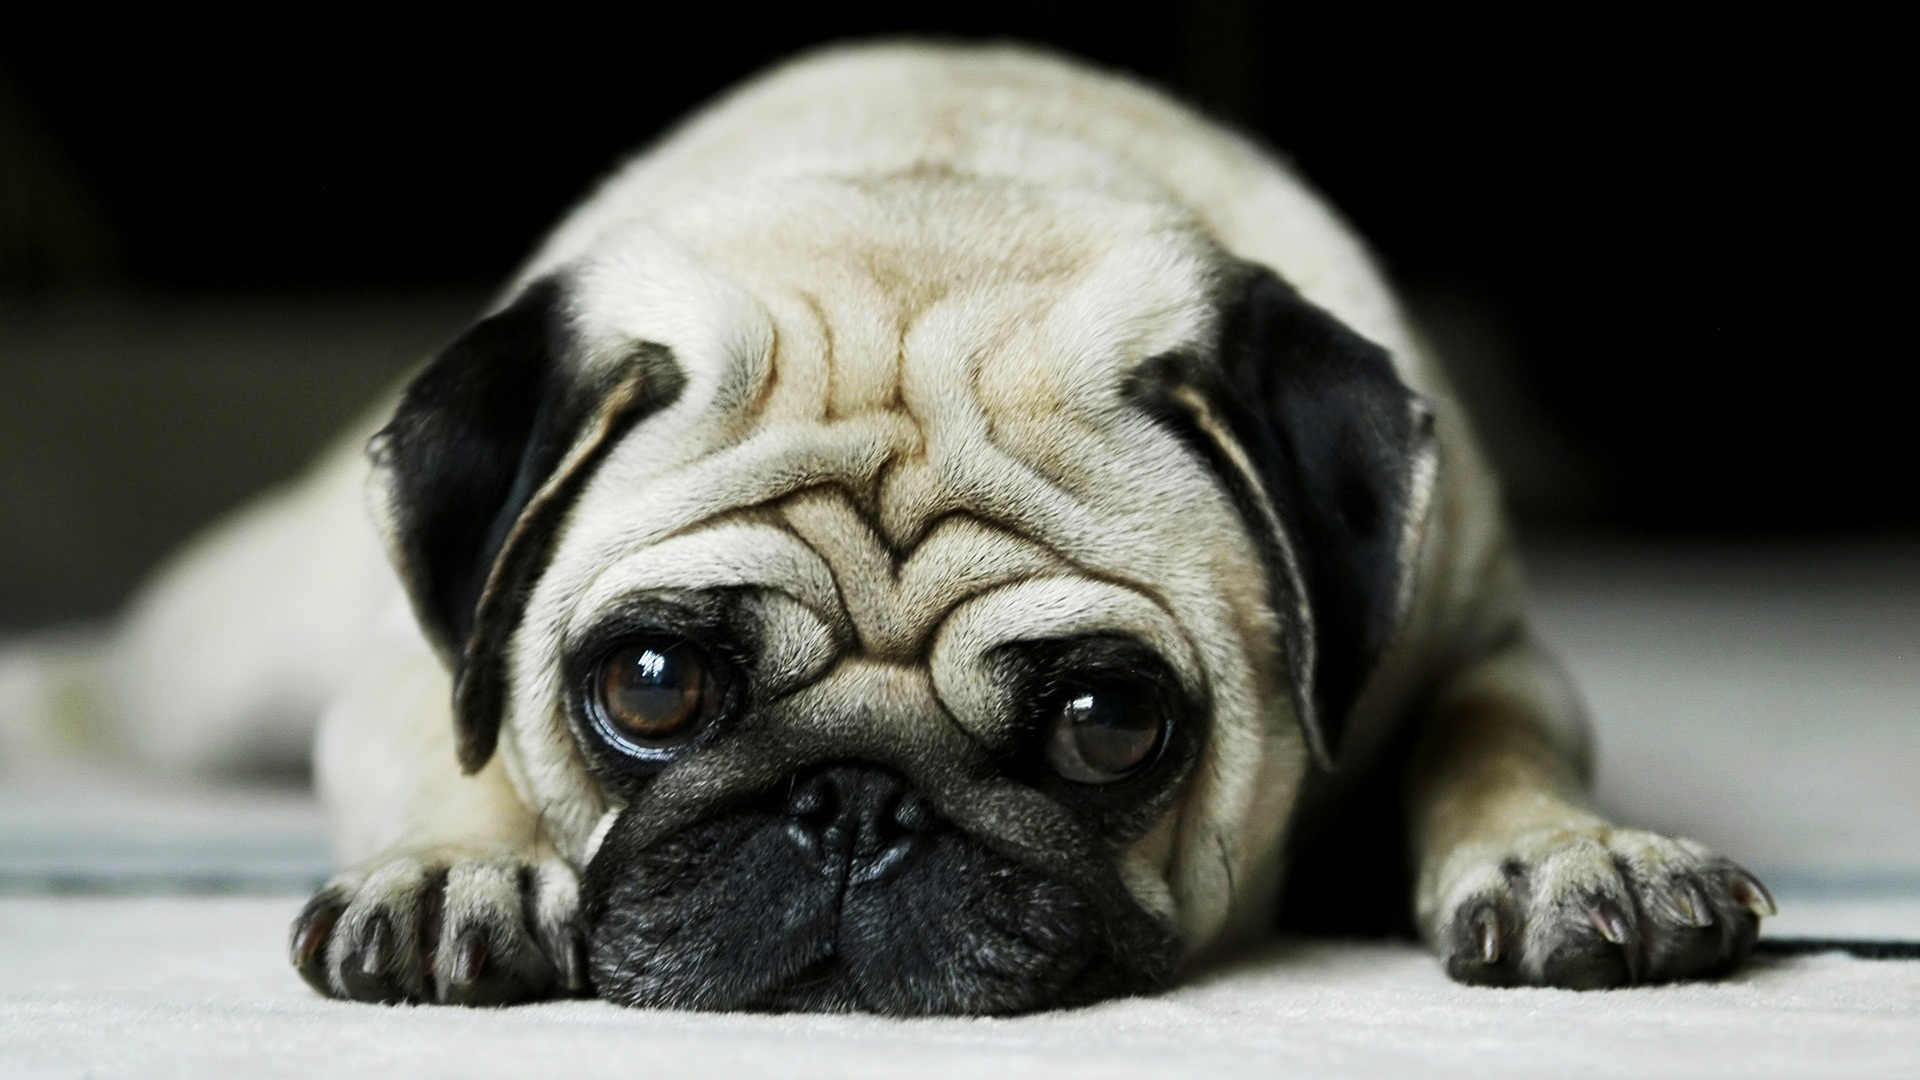
\includegraphics[scale=0.1]{example} %Example is the name of the image
			\item Interests\newline
				Fill in later...
			\item Technical Skills\newline
				Fill in later...
			\item Past experience relevant to project\newline
				Fill in later...
			\item Non-technical strengths\newline
				Fill in later...
			\item What makes you want to do the project\newline
				Fill in later...
		\end{itemize}
		\item {Shaun Meintjes (13310896)\par}
		\begin{itemize}
			\item Photo\newline
				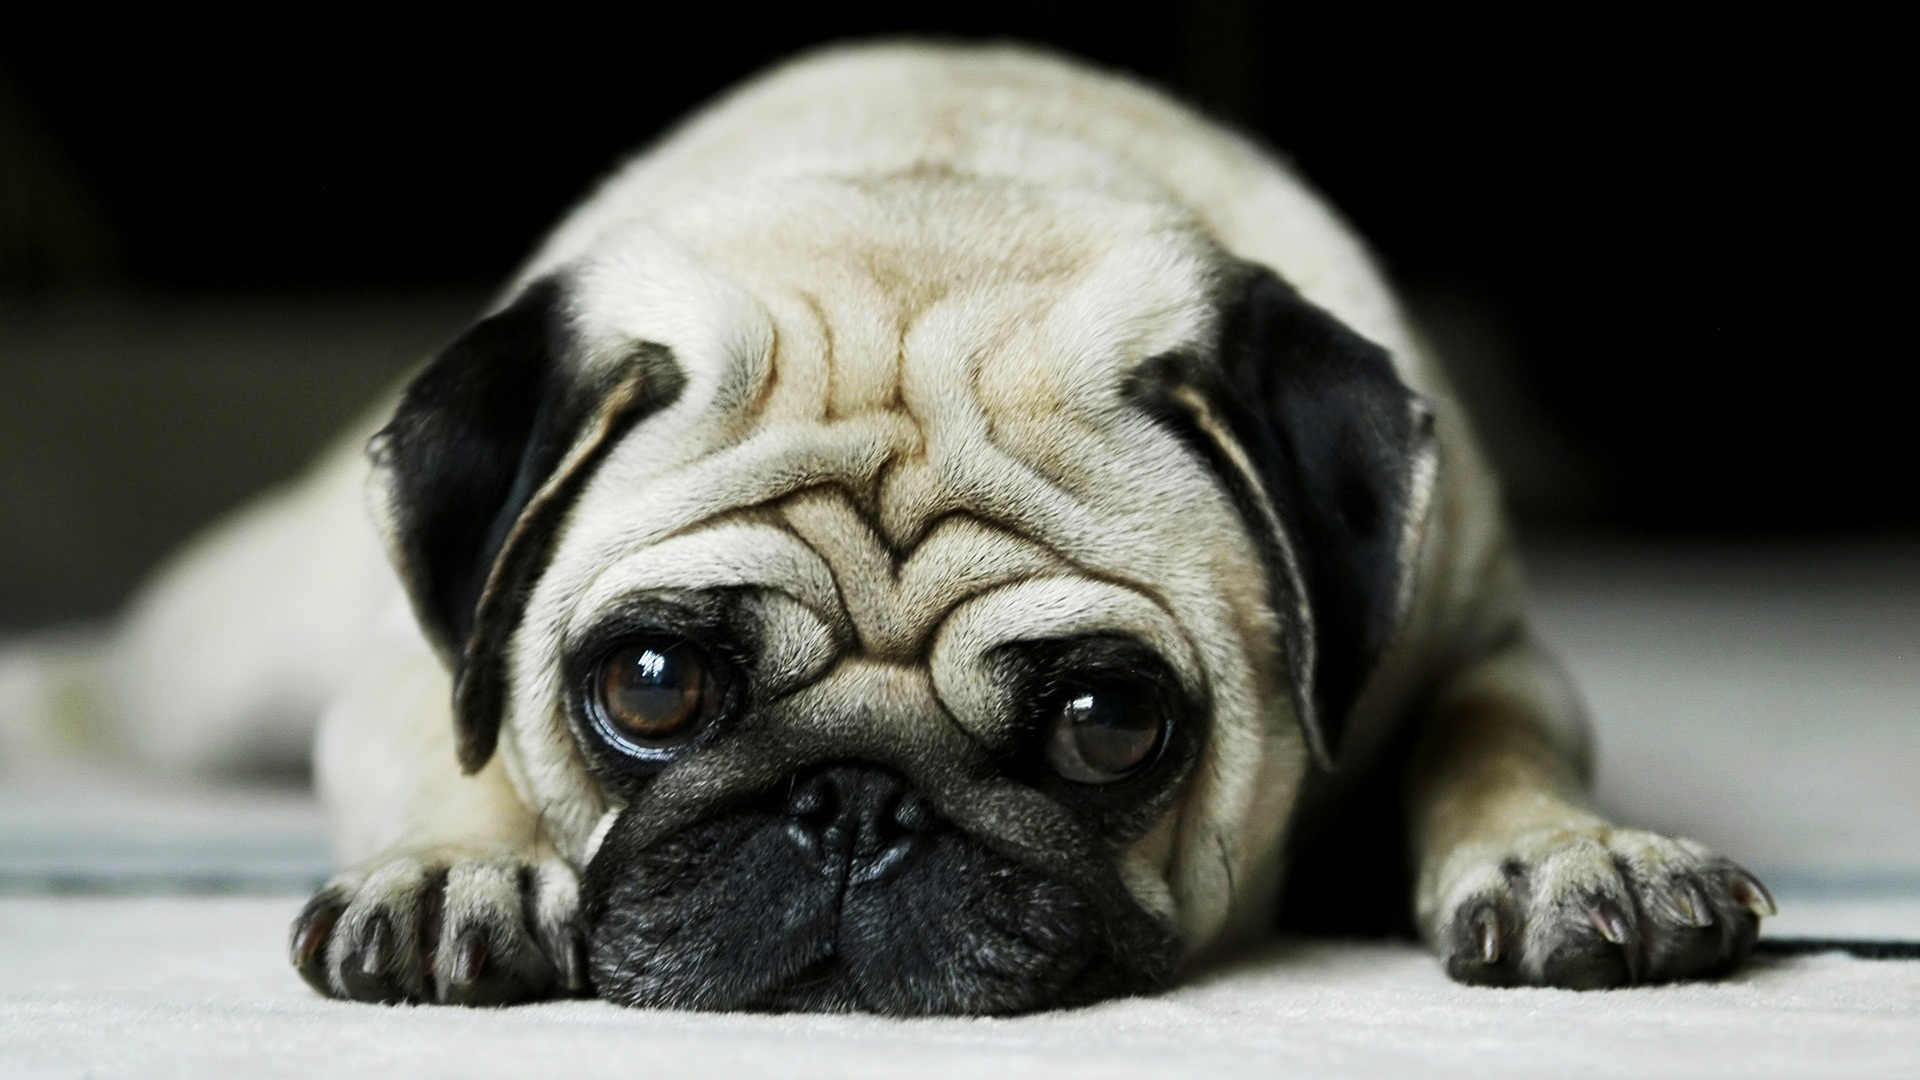
\includegraphics[scale=0.1]{example} %Example is the name of the image
			\item Interests\newline
				Fill in later...
			\item Technical Skills\newline
				Fill in later...
			\item Past experience relevant to project\newline
				Fill in later...
			\item Non-technical strengths\newline
				Fill in later...
			\item What makes you want to do the project\newline
				Fill in later...
		\end{itemize}
	\end{enumerate}
	
\section{Project Execution}
	\subsection{Development Methodology}
		Fill in later...
	\subsection{How to keep the client informed about the status of the project}
		Fill in later...
	\subsection{Initial ideas on solving some of the technical challenges}
		Fill in later...
	\subsection{Techologies we intend to use for the project}
		Fill in later...
	\subsection{What the client will receive from us at the end of the project}
		Fill in later...
	\subsection{Etc.}
		Fill in later...

\end{document}